\documentclass[12pt]{article}

% Language setting
% Replace `english' with e.g. `spanish' to change the document language
\usepackage[english]{babel}

% Set page size and margins
% Replace `letterpaper' with `a4paper' for UK/EU standard size
\usepackage[a4paper,top=2cm,bottom=2cm,left=2cm,right=2cm,marginparwidth=1.75cm]{geometry}


% Useful packages
\usepackage{amsmath}
\usepackage{graphicx}
\usepackage[colorlinks=true, allcolors=blue]{hyperref}
\usepackage{enumitem}
\usepackage{setspace}
\usepackage{wrapfig}
\usepackage{hyperref}
\usepackage{tikz}
\usepackage{outlines}
\hypersetup{
    colorlinks=true,
    linkcolor=blue,
    filecolor=magenta,      
    urlcolor=cyan,
    pdftitle={Overleaf Example},
    pdfpagemode=FullScreen,
    }


% Background
\AddToHook{shipout/background}{%
    \put (0in,-\paperheight){
\includegraphics[width=\paperwidth,height=\paperheight]{images/tausta.png}}%
    \put (0in,-\paperheight){
\includegraphics[width=\paperwidth,height=0.05\paperheight]{images/bottom.png}}%
}

% Remove indent.
\parindent 0px
\setstretch{1}


\begin{document}



\title{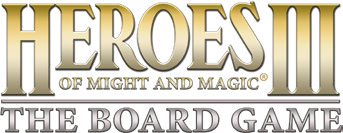
\includegraphics[width=4cm]{images/title.png} The Rewritening}

\author{Hermanni "Heegu" Karppela}
\maketitle



\begin{center}
Version 0.2
\end{center}

\tableofcontents

\clearpage

\textbf{Heroes of Might and Magic III: The Board Game} is a tactical strategy RPG board game for 1-3 players using the core box set. The continent of Antagarich is under war as several different factions, led by their heroes, battle for supremacy. Choose your faction and your hero and banish your unruly enemies from these lands.

\section{Game modes}
Each game of Heroes III is played using a scenario from the scenario book. There are four types of scenarios:
\subsection*{Clash}

A fully competitive mode for 2-3 players. 

\subsection*{Campaign}
A single player mode of interconnected scenarios against an enemy AI. For rules unique to solo mode, see \hyperlink{AIrules}{here}. Further rules changes are detailed in the campaign mission books.

\subsection*{Alliance}
A 2 vs. 2 team-based mode. You will need an expansion pack to be able to play a 4-player game. The scenarios for alliance mode can be found in any of the expansion pack rule books that add an additional faction (with the exception of the stretch goals rule book).

\subsection*{Co-op}
A cooperative mode for 2-3 players where everyone shares the same goal. 
\clearpage


\section{Setup}
This section will guide you through the process of setting up a scenario from the mission book.

\begin{enumerate}
\item Select a scenario from the mission book. For your first game we recommend that you choose the “Brave New World” scenario (see page 7 in the mission book).
\item Choose your faction from any of those not yet chosen.
\item Choose one of your faction’s heroes as your main hero. Each faction has at least one double-sided hero card, with each side depicting a different hero.
\item Take the following components belonging to your faction:
\begin{itemize}
\item[a)]1 × Double-sided hero card (on the side of the chosen hero)
\item[b)]2 × Hero model
\item[c)]7 × Town building tile
\item[d)]1 × Town board
\item[e)]7 × Double-sided unit card
\item[f)]3 × Hero-specific specialty card (of the chosen hero)
\item[g)]1 × Hero-specific ability card (of the chosen hero)
\item[h)]20 × Faction cube
\item[i)]1 × Build token
\item[j)]1 × Population token
\item[k)]1 × Spell book token
\item[l)]3 x Movement tokens
\end{itemize}
\item Place one of your faction cubes on the first space of the level tracker found on the Hero card (Represented by a “1”). Your hero is now level 1.
\item Set the game up according to the number of players and the map tile layout shown in the Mission Book.
\item Place the town board of your chosen faction in front of you and prepare the town building tiles by placing them beside the town board. Check which buildings are already built in the scenario you are about to play and place the respective building tiles on the town board. Resolve any immediate effects from already built buildings at the end of the set up.
\item Set your starting income as indicated by the scenario’s rules by placing your faction cubes on the income trackers on your town board. Place the population, build, and spell book tokens in their respective spots on the town board.
\item Group the resource tokens into separate piles located within reach of all players. Take the starting resources determined by the scenario you are playing and place them next to your town board. This is your resource pool.
\item Separate the remaining tokens into piles within reach of all players.
\item Sort the statistic cards into four piles: Attack, Defense, Power, and Knowledge. Refer to your hero statistics on your \hyperlink{Herocard}{hero card} and take the corresponding number of cards from each pile.
\item If your main hero is a hero of might, add 1 copy of the magic arrow spell to your deck, and if they’re a hero of magic, add 2 of these spells to your deck.
\item Add your hero’s ability and level 1 specialty cards to your starting deck.
\item Shuffle your starting deck and place it face down next to your hero card. Your deck is now ready for play.
\item Sort the ability, artifact, and spell cards into 3 face down decks (including any unused magic arrow spells) and shuffle them. From each of these decks, take the top card and place it face up next to its deck, creating 3 separate discard piles.
\item Choose the scenario’s \hyperlink{Difficulty}{difficulty} and take the corresponding starting bonus(es).
\item Sort the neutral Units into 4 decks according to their tier (Bronze, Silver, Gold, and Azure). Shuffle these decks individually and place them face down, leaving enough room for their discard piles.
\item Place the combat board within reach of the players. Check the scenario for which starting units you receive and place them into a pile near your town board, separate from the rest of your faction’s units.
\item Place the round tracker next to the map and place a black cube on the first space of the tracker (represented by a “1”).
\item Shuffle the astrologers proclaim cards and place them face down next to the round tracker.
\item Rotate your starting tile freely. Choose which hero model represents your main hero in this game and place the chosen hero model on the center field of your starting tile with your faction’s town.
\item Choose a starting player.

\end{enumerate}

\clearpage

\begin{center}
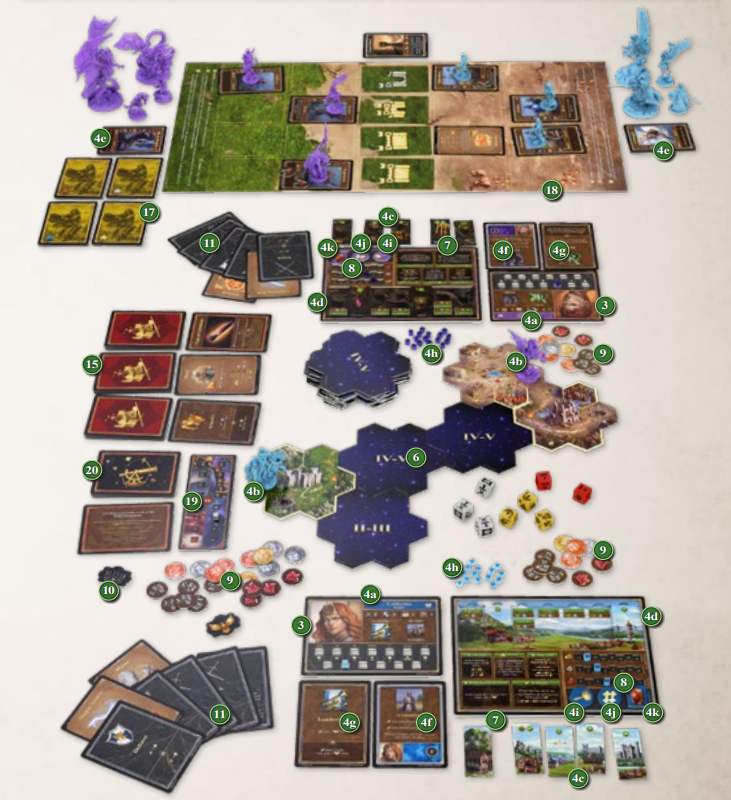
\includegraphics[scale=0.9]{images/setup.PNG}
\end{center}

\clearpage

\section{Round structure}
The game is structured into rounds, during which each player will take their own turn in a clockwise order starting with the starting player. During their turns, players will move their \hyperlink{Heroes}{heroes} on the game map, construct new buildings in their \hyperlink{Town}{town} and recruit \hyperlink{Units}{units} in an attempt to fulfill the scenario’s victory condition.\\[6pt]
Perform the following steps at the start of every round except the first one:
\begin{itemize}
\item Flip any previously used build, population and/or spell book tokens back to their active side.
\item Flip any previously used movement point (MP) tokens back to their active, green side.
\item Regain uses for expert effects.
\end{itemize}
Then, depending on the current round number, players either gain resources or resolve an astrologers proclaim card:
\begin{itemize}
\item Odd-numbered rounds are resource rounds. All players gain income from the buildings, settlements, and mines they control. Skip this step during the first round.
\item Even-numbered rounds are astrologers’ rounds. Draw an astrologers proclaim card and resolve its effects.
\item If the scenario has timed events marked on the round tracker that have now been reached, resolve them.
\end{itemize}
\subsection*{Player actions}
\begin{itemize}
\item During their turn, players spend their movement points (MP) to perform actions with their heroes.
\item Build, population and spell book tokens may be used at any point during any player’s turn except during combat.
\item Once all players have performed their turn, move the black cube on the round tracker and perform the start of round phase for the next round.
\end{itemize}
Keep playing new rounds until any of the scenario’s ending conditions have been met.

\clearpage

\section{Player turns}
At the start of a player’s turn, that player refreshes their hero's hand of cards from their deck following two steps in order:
\begin{itemize}
    \item Discard any number of cards from your hand. If your current hand exceeds your hand limit, you must discard down to at least your hand limit.
    \item Draw back to your hand limit.
\end{itemize}
Your current hand limit depends on your hero’s \hyperlink{Level}{level}. The beginning of your turn is the only time your hand size is checked.\\[6pt]
There are three types of actions players may take during their turn:
\subsection*{Movement actions}
Movement actions are performed by using movement points. A player can use movement actions only during their own turn.\\[6pt]
For every 1 MP spent, you can perform one of the following actions:
\begin{itemize}
    \item Move a hero 1 field in any direction.
    \item \hyperlink{Categories}{Re-visit} a field where your hero is in.
    \item \hyperlink{Timelimit}{Continue combat} against neutral units for 1 additional round.
    \item \hyperlink{Placing}{Discover a face down map tile} if the hero is on a field next to that map tile.
    \item Place a new map tile from your pool of far (II-III) map tiles.
\end{itemize}
Mark the amount of MP you have used by flipping your movement tokens over to their brown, inactive side. If a player has both a main and a secondary hero, track their MP separately. Heroes can spend MP in any order.\\[6pt]
Allied heroes can move through each other but cannot stop their movement in the same field. When you move through a field with an allied hero, do not visit the field that the allied hero is standing on. In the unlikely situation that two allied heroes are forced onto the same field, you must use your next MP to move one of them away from that field.\\[6pt]
\begin{figure}[h]
\centering

\includegraphics[width=0.25\linewidth]{mp.png}
\end{figure}\\
\begin{center}
\textit{An active and an inactive movement token.}
\end{center}




\clearpage

\subsection*{Town actions}
You can perform each of the town actions listed below \textbf{once per round}. These actions can be performed at any point during any player’s turn, except during combat or when a player is resolving an action that would be interrupted by your town action. For example, you cannot draw spell cards simultaneously with the spell book token.\\[6pt]
When a player announces that they are about to start combat, you may react to it with a town action before performing any of the steps of \hyperlink{Combatsetup}{setting up combat.}\\[6pt]
If multiple players wish to use a town action at the same time and the order of resolving them has an effect on the game, you may roll an attack or resource die and let the highest roller perform the action first.\\[6pt]
After performing a town action, flip the respective token on its inactive side on your town board. You cannot use that action again until the start of the next round, when the tokens are refreshed.
\begin{itemize}
\item Build token, used to expand your \hyperlink{Town}{town}.
\includegraphics[scale=0.5]{build.png}
\item Population token, used to recruit and reinforce \hyperlink{Units}{units} or to recruit \hyperlink{Secondary}{a secondary hero}.
\includegraphics[scale=0.5]{images/population.PNG}
\item Spell book token, used to purchase \hyperlink{spells}{spells}.
\includegraphics[scale=0.5]{images/spells.PNG}
\end{itemize}

\subsection*{Morale actions}
Players can gain or lose morale through various game effects. When a player gains morale, place a positive morale token 
\includegraphics[scale=0.75]{images/positive.PNG} near your play area. A player may only have one such token. If they would gain a second token, they may immediately spend the first one before gaining the second. A positive morale token may be spent to perform any of the following actions at any time:
\begin{itemize}
\item Draw a card from your hero's deck.
\item Discard any number of cards, then draw that many cards.
\item Reroll any die you have thrown.
\end{itemize}
If a player loses morale, they must discard a positive morale token 
\includegraphics[scale=0.75]{images/positive.PNG} without effect if they have one, otherwise they gain a negative morale token 
\includegraphics[scale=0.75]{images/negative.PNG}. Gaining morale while you have a negative morale token discards the negative morale token without effect. If a player would gain a second negative morale token, they must instead discard their entire hand of cards the next time they end their turn.\\[6pt]
\textbf{NOTE:} The Necropolis faction ignores any morale effects. They cannot ever gain or lose morale for any reason.\\[12pt]
Once all players have spent all their movement points on their turns and do not wish to use any further town or morale actions or instant effects, the current round is over.\\[6pt]

\clearpage

\section[Heroes]{Heroes\hypertarget{Heroes}{}}
Players always control a main hero and may additionally also recruit a secondary hero. A “player’s hero” may refer to either of them. Heroes are used to perform movement actions on the game board and to start combats against enemies in order to reach a scenario victory condition. Whenever a hero gains a card for any reason, put it directly into your hand unless otherwise stated. 
\subsection*{Main hero}
The main hero is represented by its chosen model and hero card. Each faction’s main hero has 3 movement points. Only the main hero can use its own deck of cards.\\[6pt]
Each main hero starts the game at level 1 and can advance up to level 7 by gaining experience. Experience is gained from winning combat, visiting certain locations and the treasure die. Gaining 1 experience is represented by the symbol 
\includegraphics[scale=0.75]{images/exp.PNG}. \hyperlink{Level}{Leveling up} provides the hero various benefits. \hyperlink{Units}{Units} owned by the player may always participate in combat started in the same field as their main hero.
\subsection*{\hypertarget{Secondary}{Secondary heroes}}
If you control a town or a settlement, a secondary hero can be hired by flipping your population token and paying 10 gold. \textbf{Note}: Units cannot be \hyperlink{Units}{recruited or reinforced} during that use of the population token.\\[6pt]
Your secondary hero uses the remaining hero model of your faction. You may wish to mark this model with a token such as a faction cube to differentiate it from the main hero. After hiring a secondary hero, place the model in a town or settlement you control. You can only have one secondary hero at a time.\\[6pt]
Secondary heroes have 2 movement points. They do not have their own hero card, cannot gain experience, and cannot use your main hero's deck for any reason. If a secondary hero gains any cards, place them into your hand as normal.
Secondary heroes are considered to have the same level as the main hero for the purposes of resolving \hyperlink{Quick}{quick combat} against neutral enemies.\\[6pt]
Units owned by the player may always participate in combat started in the same field as their secondary hero.\\[6pt]
If your secondary hero is attacked by an enemy hero, you can choose to have your hero be \hyperlink{Endcombat}{instantly defeated instead of fighting a combat}. When a secondary hero is defeated, remove them from the game. They can be recruited again with another use of the population token.\\[6pt]

\clearpage

\begin{wrapfigure}{r}{0.5\textwidth}
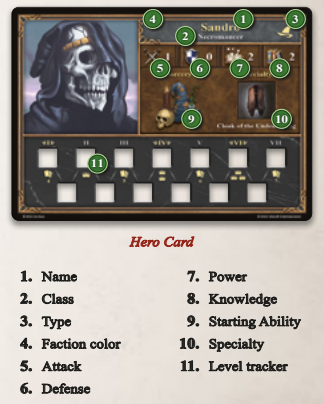
\includegraphics[width=0.9\linewidth]{images/herocard.PNG} 
\end{wrapfigure}
\subsection*{\hypertarget{Herocard}{Hero card anatomy}}
\begin{enumerate}
\item Name – The hero’s name. Used for identification. Has no gameplay effect.
\item Class – The hero’s class. Has no gameplay effect.
\item Type – The hero’s type (might 
\includegraphics[scale=0.3]{images/might.PNG} or magic 
\includegraphics[scale=0.3]{images/magic.PNG}). Determines the amount of magic arrow spells in your starting deck (1 or 2 respectively).
\item Faction color – Reminder for the color of the faction’s cubes and miniatures.
\item Attack – Number of attack cards in your starting deck.
\item Defense – Number of defense cards in your starting deck.
\item Power – Number of power cards in your starting deck.
\item Knowledge – Number of knowledge cards in your starting deck.
\item Starting Ability – Reminder for the unique ability card the hero starts with.
\item Hero Specialty – Reminder for the specialty cards the hero adds to their deck at the start of the game and after specific level ups. Each hero has three specialty cards.
\item Level - Whenever a main hero gains 1 or more experience 
\includegraphics[scale=0.75]{images/exp.PNG} move the cube that number of steps on this track. When the cube reaches the next slot on the upper row, the hero gains a level.
\end{enumerate}
\clearpage

\subsection*{\hypertarget{Level}{Level effects}}
The most common sources of gaining experience are the treasure die and \hyperlink{Combatexperience}{combat}. Each new level up requires 2 experience. When a main hero reaches a new level, resolve the effects of the level up immediately. If a main hero gains multiple levels at the same time, resolve the effects in ascending level order. Gaining experience at level 7 has no effect.\\[6pt]
The level tracker on your hero card shows the following information:
\begin{itemize}
\item Your main hero’s current level and amount of experience gained, shown by the cube's position.
\item Your current hand limit 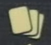
\includegraphics[scale=0.5]{images/hand.PNG}.
\item The number of \hyperlink{Ability}{expert effects} 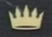
\includegraphics[scale=0.5]{images/expert.PNG} you may use during a round. Track the number of uses each player has in any suitable manner, such as by moving black cubes on and off your hero card.
\item At which levels your main hero must search for a new \hyperlink{Ability}{ability card} or gain a \hyperlink{Specialty}{specialty card}. Level numbers written in gold on the level tracker (1, 4 and 6) give you a specialty card, while silver levels (2, 3, 5, 7) give you an ability card.
\end{itemize}
List of all effects:
\begin{itemize}
\item \textbf{Level 1} – Your hand limit is 4. Add your first specialty card to your deck.
\item \textbf{Level 2} – Search (2) the ability deck. You may play 1 card for their expert effect per round.
\item \textbf{Level 3} – Your hand limit is 5. Search (2) the ability deck.
\item \textbf{Level 4} – Gain your second specialty card. You may play 2 cards for their expert effect per round.
\item \textbf{Level 5} – Your hand limit is 6. Search (2) the ability deck.
\item \textbf{Level 6} – Gain your third specialty card. You may play 3 cards for their expert effect per round.
\item \textbf{Level 7} – Your hand limit is 7. Search (2) the ability deck.
\end{itemize}

\clearpage
\subsection*{\hypertarget{Playerdecks}{Player decks}}
All players have a unique deck which represents their main hero's abilities and equipment. Decks may contain statistic cards, ability cards, spell cards, artifact cards and the chosen hero’s specialty cards. Whenever a player gains a new card, they always place it directly into their hand unless otherwise stated. Each player’s deck starts with 9 cards, built during the game’s set up.
\subsection*{General card rules}
\begin{enumerate}
    \item Whenever you are instructed to \textbf{search} (X) the ability, artifact, or spell deck, you may either look at the top (X) cards from the specified deck, take one of them to your hand, and discard the others, or-instead of looking at the top (X) cards add the top card from that deck’s discard pile to your hand.
    \item The ability, artifact, and spell decks each have their own discard piles, created during the setup, which help players identify these decks. If a deck ever runs out of cards, reshuffle it and discard its top card to form a new discard pile. Also, whenever an ability, artifact or spell deck discard is empty, refill it with that deck’s top card.
    \item Whenever you are instructed to remove a card, remove it completely from the game and return it to the box.
    \item Player cards have the following types of effects:
    \begin{itemize}
        \item \textbf{Instant} 
\includegraphics[scale=0.75]{images/instant.PNG} effects are resolved immediately and can be played out of turn.
        \item \textbf{Activation} 
\includegraphics[scale=0.75]{images/activation.PNG} effects must be played when activating a unit in combat.
        \item \textbf{Map} 
\includegraphics[scale=0.75]{images/map.PNG} effects must be played on your turn and cannot be used during combat.  
        \item \textbf{Ongoing} 
\includegraphics[scale=0.75]{images/ongoing.PNG} effects must be played on your turn and last until they are used up or until the player who played them starts their next turn (whichever happens first).
        \item \textbf{Permanent} 
\includegraphics[scale=0.5]{images/permanent.PNG} effects must be played on your turn and stay in your play area until discarded or replaced. Players may have only one permanent card at a time; playing another discards the first.
    \end{itemize}
    \item After a card is used, discard it. Each player has their own separate discard pile for their own deck.
    \item If your hero's deck is empty when you need to draw a card, shuffle your discard pile into a new deck.
\end{enumerate}

\clearpage
\subsection*{\hypertarget{Ability}{Ability and statistic cards}}
\begin{wrapfigure}{R}{0.5\textwidth}
 
    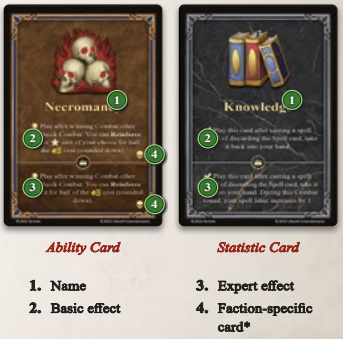
\includegraphics[width=0.48\textwidth]{images/ability.PNG}

\end{wrapfigure}
Every ability and statistic card has a basic effect and a stronger expert effect, which is shown below the basic effect. Whenever a player plays an ability or statistic card, they must choose which effect they are using. The number of expert 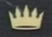
\includegraphics[scale=0.5]{images/expert.PNG} effects a player can use each round is limited by their main hero’s \hyperlink{Level}{level}.\\[6pt]
\textbf{Important}: Certain cards are limited to the Necropolis faction 
\includegraphics[scale=1]{images/necro.PNG}. When a non-Necropolis player draws one, they may either discard it and draw a new card as a replacement or gain it as normal. Non-Necropolis players cannot use faction specific cards from their hand in any way besides discarding them.
\subsection*{Artifact cards}
Artifact cards are divided into 3 levels: minor, major, and relic. These levels relate to the overall power of the card and may be referenced when resolving certain effects or during scenario set up. Artifacts are gained through map exploration.\\[6pt]
If you gain an artifact as part of applying the difficulty bonus during a scenario’s set up, keep it in your hand instead of shuffling it into your deck.
Artifacts can be \hyperlink{Trading}{traded} in alliance and cooperative scenarios.\\[6pt]
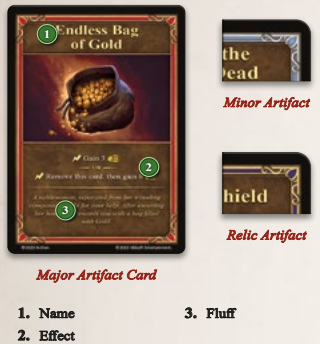
\includegraphics[scale=1]{images/artifact.PNG}

\clearpage

\subsection*{\hypertarget{spells}{Spell cards}}
\begin{wrapfigure}{R}{0.5\textwidth}
    \begin{center}
    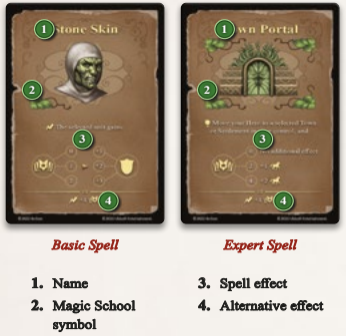
\includegraphics[width=0.48\textwidth]{images/spell_example.PNG}
    \end{center}
\end{wrapfigure}
Spell cards have three possible primary effects. Using the topmost basic version of the spell has no additional costs. Accessing the second and third effects requires the spell to be \textbf{empowered} before it is played. The amount a spell needs to be empowered for each effect is indicated within a circle in the middle of its card text.\\[6pt]
You may empower a spell by playing any card for its empower 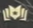
\includegraphics[scale=0.75]{images/empower.PNG} effect. The bottom, alternative effect of all spell cards is to empower another spell.\\[6pt]
\textbf{Important}: During combat, \textbf{only one spell} card may be played by each player \textbf{per combat round}.\\[6pt]
Spells can be gained by building the mage guild. When you do, search (2) the spell deck, twice. If you start a scenario with the mage guild, perform the searching in turn order and shuffle the cards into your deck at the end of the set up. More spells can be bought by flipping your spell book token and paying the indicated cost on the guild to search (2) the spell deck. This cannot be done during the same round as when the guild is constructed. Spells can be \hyperlink{Trading}{traded} in alliance and cooperative scenarios.

\subsection*{\hypertarget{Specialty}{Hero specialty cards}}
Hero specialty cards are gained from level ups. Each hero has an unique set of them. While many specialty cards have effects which resemble spell cards, specialty cards are their \textbf{own unique category of card}, which are not affected by effects that do not specifically specify them.
\\[6pt]

\begin{figure}[h]
\centering
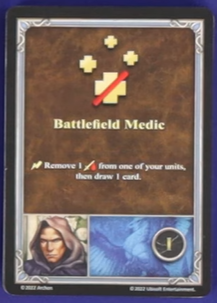
\includegraphics[width=0.25\linewidth]{images/specialty.PNG}
\end{figure}
\begin{center}
\textit{A level 1 specialty card, belonging to Rion the cleric.}
\end{center}

\clearpage
\section{Resources}
There are three types of resources in the game: gold, building materials, and valuables.
Resources are spent during the game to expand your town, to recruit units, and to purchase spells. You can gain resources from settlements and mines that you have \hyperlink{Categories}{flagged}, but also by using artifacts and rolling resource dice 
\includegraphics[scale=0.75]{images/resource_die.PNG}. Whenever a player's resource production is increased or decreased, move that resource's cube on its production track the appropriate number of spaces.\\[6pt]

\includegraphics[scale=1]{images/resources.PNG}\\
Players start each scenario with the number of resources indicated in that scenario’s set up.
Resources are also gained at the start of each resource round. When they are gained or spent, exchange the appropriate number and type of resource tokens between your faction's and the game's supply. Resources can also be \hyperlink{Trading}{traded}. There's no limit to the amount of resources you can have.
\section[Town]{Town\hypertarget{Town}{}}
Each faction has their own town, which is located in the center of their starting tile. The town is your most important location, as many scenarios \hyperlink{End}{may end} if it's flagged by an enemy hero.\\[6pt]
The contents of your town and overall faction status are represented by the town board. The board shows your currently built buildings, resource costs for future buildings, your resource incomes and status of town tokens.\\[6pt]
All factions are able to build the following buildings in their town:
\begin{itemize}
    \item \textbf{City hall} – Provides resource income or a faction-specific ability.
    \item \textbf{Citadel} – Allows you to reinforce units when using the population token. Also \hyperlink{Walls}{protects your town} when it is attacked.
    \item \textbf{Unit dwellings} – Allows you to recruit units. Dwellings have three levels that unlock new units, but which must be built in the following order:
\includegraphics[scale=0.75]{images/levels.PNG}
    \item \textbf{Mage guild} - gives you \hyperlink{spells}{spells}.
    \item \textbf{Faction building} - a faction-specific building with a unique effect.
\end{itemize}
\textbf{A single building} may be constructed each round by using the build token. When you construct a building, pay its cost in resources, flip the build token to its inactive side, and place the new building’s cardboard piece into its proper slot on the town board. If the building has any immediate effects upon building it, resolve them now.\\[6pt]
If a town or settlement is attacked by an enemy hero and your hero is not also on that field, you may immediately \textbf{pay 8 gold} to fight a defending combat using only your units. You cannot use your deck during that combat as your main Hero is not present. Paying this gold represents the cost of transporting the army there.\\[6pt]
When you flag a town, take \hyperlink{End}{a faction cube} from its previous owner.

\clearpage

\begin{wrapfigure}{r}{0.5\textwidth}
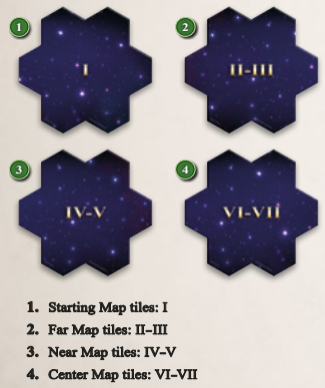
\includegraphics[width=0.9\linewidth]{images/maptiles.PNG} 
\end{wrapfigure}
\section{Map locations}
Each scenario is built using four types of map tiles. Players always have a faction-specific starting (I) map tile and may additionally have a number of face-down far (II-III) map tiles which can be used to add new areas to the scenario by spending MP. Near (IV-V) and center (VI-VII) tiles are usually placed face-down during a scenario’s set up and must be turned face up by spending MP.\\[6pt]
The roman numeral of each tile describes the overall difficulty of neutral armies on that tile, as well as the number of rewards players might expect to find on that tile. Starting (I) tiles are the easiest while center (VI-VII) tiles are the most difficult.\\[6pt]
During a scenario’s set up, you will be instructed to use a certain amount of specific map tiles. Follow the scenario’s set up instructions and gather the necessary tiles. All face-down tiles should be selected randomly from the pool of possible tiles and shuffled to keep their front side hidden.\\[6pt]
\begin{wrapfigure}{R}{0.5\textwidth}
    \begin{center}
    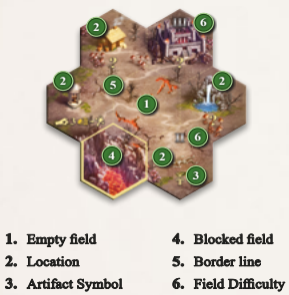
\includegraphics[width=0.48\textwidth]{images/fields.PNG}
    \end{center}
\end{wrapfigure}
\subsection*{Map tile anatomy}
Each map tile is divided into 7 separate \textbf{fields} that your heroes can \textbf{visit}. When a hero moves to a field, they must immediately visit it, or 
first start a \hyperlink{Combat}{combat} against neutral enemies or another player depending on the tile they have just entered. If the hero wins the combat, they must then visit that field afterwards. Visiting fields provides heroes with benefits such as gaining resources or cards. Empty fields do nothing when visited. Solid yellow lines on a field's edge cannot be passed through. \hyperlink{Difficulty}{Roman numerals} indicate that a field is guarded by neutral enemies that must be fought.\\[6pt]

\clearpage
\subsection*{\hypertarget{Categories}{Location categories}}
There are three categories of visitable fields:
\begin{itemize}
    \item \textbf{Visitable} – Once you visit this field place a black cube on it. Treat it as an empty field as long as it has a black cube.
    \item \textbf{Flaggable} – These fields can be directly captured by players. When you visit it, place one of your faction cubes on it and gain a benefit. Enemy heroes who visit your flagged fields will replace your cube with theirs to steal the field’s effects. Allied heroes treat flagged fields as if they were empty.
    \item \textbf{Revisitable} – You can visit this field multiple times. Do not place a black cube when you visit it. You may pay 1 MP to visit this field again when your hero occupies this field.
\end{itemize}

See \hyperlink{All}{this section} for a list of all possible fields and what they do.
\subsection*{\hypertarget{Placing}{Placing and discovering new tiles}}
When you hero is adjacent to an undiscovered face down tile, that hero may spend 1 MP during your turn to turn that tile over. You may then rotate the tile as you see fit and place it face-up. That tile can now be moved onto normally.\\[6pt]
In some scenarios you will receive your own individual stack of far (II-III) map tiles. These can be placed on the map to expand the play area. Players may only use the tiles they were given during set up. Tiles should be kept hidden from everyone until they are about to be placed.\\[6pt]
Placing a new tile costs 1MP. The new tile must be adjacent to the hero who spends the MP, and to at least two other existing tiles. New tiles must also be positioned so that there is a valid path that eventually joins them with all other tiles. You may always rotate map tiles when placing them.\\[6pt]
\begin{center}
    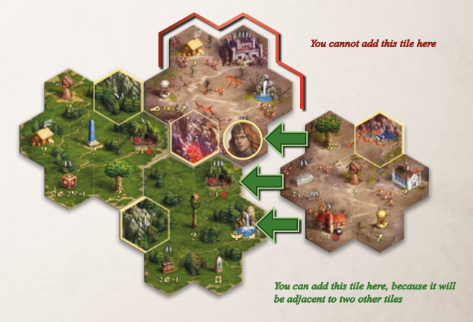
\includegraphics[scale=1]{images/placement.PNG}
\end{center}


\clearpage
\section[Units]{Units\hypertarget{Units}{}}

In addition to their hero and its deck, players have a deck of unit cards which represent the armies moving with their heroes. Every faction has access to 7 different units, each with unique stats and abilities. Units are necessary for winning combats and fulfilling scenario goals. Each scenario's set up instructions indicate which unit cards should be included in your initial unit deck. Your current unit deck should be kept near the town and hero boards, clearly separated from the rest of your faction’s units.\\[6pt]
Each faction unit is double-sided, with a weaker “Few” side, and a stronger “Pack” side. “Few” units may be upgraded to “Packs” by \textbf{reinforcing} them, while taking damage in combat can subsequently reduce a unit back to its “Few” side. Units should always be kept on their correct side when moved around or inspected.\\[6pt]
A player’s unit deck may have any number of units, but only up to 5 units can be selected to fight during \hyperlink{Combatsetup}{combat set up}. If a unit is defeated in combat, remove it from your unit deck. After combat, return any surviving units to your unit deck. Defeated faction units can be recruited again after being defeated. Units may be recruited and reinforced by flipping the population token and paying the unit's recruitment 
\includegraphics[scale=0.25]{images/pay.PNG} or reinforcement 
\includegraphics[scale=0.25]{images/reinforce.PNG} cost. When you do so, you can instantly recruit and reinforce \textbf{any number} of times, provided you have enough resources and the prerequisite buildings to do so.\\[6pt]
\textbf{Recruiting} a unit requires that your town has a dwelling of that unit’s level or higher. \textbf{Reinforcing} requires that your town has a citadel in addition to a dwelling of that unit’s level or higher. If you ever lose all units in your unit deck, \textbf{immediately} replace your unit deck with the starting units of the scenario.\\[6pt]
\textbf{Important}: Any effects which allow you to reinforce outside of using the population token \textbf{do not} require owning a citadel or the appropriate level of dwelling.
\begin{figure}[h]
\centering
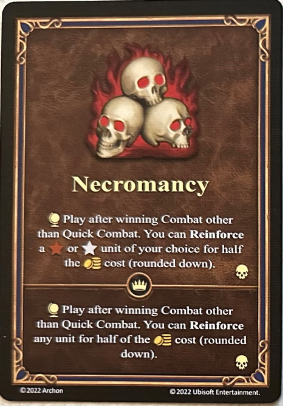
\includegraphics[width=0.25\linewidth]{images/necromancy.PNG}
\end{figure}
\begin{center}
\textit{Cards such as Necromancy allow you to reinforce outside of using the population token. This does not require owning any of the prerequisite buildings for reinforcing nor flipping your population token.}
\end{center}

\clearpage
\begin{wrapfigure}{R}{0.5\textwidth}
    \begin{center}
    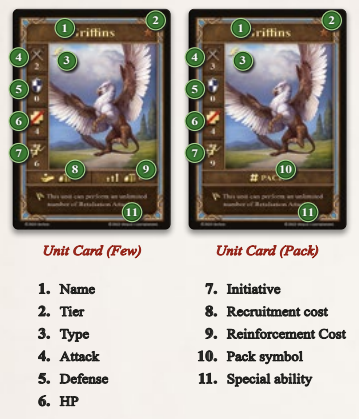
\includegraphics[width=0.48\textwidth]{images/units.PNG}
    \end{center}
\end{wrapfigure}
\subsection*{Unit card anatomy}

\includegraphics[scale=1]{images/attack.PNG}\textbf{Attack} – The amount of damage this unit deals when it attacks. Attacks are always reduced by the defending unit’s defense. Attacks may be modified by various effects such as the attack die and statistic cards.\\[6pt]

\includegraphics[scale=1]{images/defense.PNG}\textbf{Defense} - The amount by which the unit reduces the attack damage it receives. Does not apply to damage received from spells or other non-attack effects. Defense may be modified by various effects such as statistic cards.\\[6pt]

\includegraphics[scale=1]{images/HP.PNG}\textbf{\hypertarget{HP}{HP}} - The maximum amount of damage a unit can sustain before it is defeated. ”Few” units are removed from combat and its owner’s unit deck when defeated. ”Pack” units are turned back to ”Few” units, with any excess damage placed on its ”Few” side. After combat, all damage is removed from all units. Units retain their ”Few” or ”Pack” status after combat. Defeated neutral units are placed into their respective discard pile.\\[6pt]

\includegraphics[scale=1]{images/initiative.PNG}{\hypertarget{Initiative}{\textbf{Initiative}}} - Determines when the unit activates during combat. Units with a higher initiative activate first. In case of a tie, the \hyperlink{Combatterminology}{attacking} side’s unit should always activate first. If there are multiple ties on one side, the player who controls those units selects which unit to activate next. If there are multiple ties on both sides (for instance two attackers and two defenders with the same initiative), alternate between the attackers and defenders starting with the attacker.\\[6pt]
Most units have a \textbf{special ability}:\\[6pt]
  \begin{minipage}{.6\textwidth}
    \begin{itemize}[wide]
      \item\textbf{Activation} 
\includegraphics[scale=0.25]{images/unit_activation.PNG} resolves when the unit is activated.
      \item\textbf{Attack} 
\includegraphics[scale=0.25]{images/unit_attack.PNG} resolves when the unit attacks during its activation. In case of multiple attacks, resolve the effect for the first attack only.
      \item\textbf{Other} 
\includegraphics[scale=0.25]{images/unit_other.PNG} may be resolved instead of the unit's normal activation. Replaces all movement and/or attacking.
    \end{itemize}
  \end{minipage}
  \begin{minipage}{0.5\textwidth}
    \begin{itemize}[wide]
      \item\textbf{Passive} 
\includegraphics[scale=0.25]{images/unit_passive.PNG} resolves whenever its condition is met.
      \item\textbf{Retaliate} 
\includegraphics[scale=0.25]{images/unit_retaliate.PNG} resolves when the unit retaliates.
      \item In any cases without one of the above icons, the unit’s ability is used according to its text. Units may also have \hyperlink{Playerdecks}{these} symbols.
    \end{itemize}
  \end{minipage}

\clearpage
\subsection*{\hypertarget{Unittype}{Unit types}}
There are thee types of units:
\begin{itemize}
    \item \textbf{Ground} 
\includegraphics[scale=0.25]{images/unit_ground.PNG} units move up to 3 spaces and attack adjacent enemies.
    \item \textbf{Flying} \includegraphics[scale=0.25]{images/unit_flying.PNG} units move up to 3 spaces, ignoring obstacles, and attack adjacent enemies.
    \item \textbf{Ranged} \includegraphics[scale=0.25]{images/unit_ranged.PNG} units may attack any unit anywhere OR move up to 1 space.
\end{itemize}
If a \textbf{ranged} unit is next to an enemy unit, its attack target must be that adjacent enemy. When attacking an adjacent enemy in this way \textbf{or} an enemy in the backline while the ranged unit is also in its own backline, the ranged unit suffers a combat penalty. Throw two combat dice and \textbf{apply the smaller result}. Walls and gates may also \hyperlink{Walls}{reduce} a ranged unit's attack.
\subsection*{Neutral units}
Neutral units guard the various locations on the game map. Starting and winning combat against them is necessary to visit most locations. Neutral units are spread into four different tiers, each with their own deck. In addition to bronze, silver and gold, there are also azure \includegraphics[scale=0.25]{images/azure.PNG} neutral units which are the strongest in the game.\\[6pt]
Each of these decks should be kept separate from each other and shuffled during set up. If a neutral unit deck ever runs out of cards, reshuffle the discard into a new deck. When a combat against neutral units starts, \hyperlink{Difficulty}{the appropriate number} of units from each tier should be drawn to take part in that combat.\\[6pt]
It is possible for players to gain neutral units to their unit deck through various effects, such as scenario-specific rules or the diplomacy ability card. Neutral units cannot be reinforced, as they are single sided. Whenever a neutral unit is defeated from your unit deck, place it into the neutral discard pile as normal.
\begin{figure}[h]
\centering
\includegraphics[scale=1]{images/unit_list.PNG}
\end{figure}
\begin{center}
\textit{A graph of all faction units in the core game.}
\end{center}

\clearpage
\section[Combat]{Combat\hypertarget{Combat}{}}
Combat starts whenever heroes encounter enemy heroes or units, and takes place on the separate combat board. Combat with \textbf{neutral units} starts when a hero moves to an unvisited field with a \hyperlink{Difficulty}{difficulty} rating. Combat with \textbf{another player} can start in two ways:
\begin{itemize}
    \item You move into the same field as their hero.
    \item You move into a town or settlement owned by another player without their hero. If they wish to defend that field, they must \hyperlink{Town}{pay to move their army there}.
\end{itemize}
Players are able to start multiple combats during their turn.
\begin{wrapfigure}{R}{0.5\textwidth}
    \begin{center}
    \includegraphics[width=0.48\textwidth]{images/combat_board.PNG}
    \end{center}
\end{wrapfigure}
\subsection*{\hypertarget{Combatsetup}{Combat setup}}

Combat takes place on the 4 x 5 combat board, which consists of two backlines and two frontlines on opposite ends and a middle row. Follow these steps when fighting against \textbf{neutral units}:

\begin{itemize}
 \item Choose one of the combat board’s sides as your own. Place up to 5 of your unit cards freely onto the back- and frontline of that side.
  \item Check the difficulty table and draw the corresponding number of neutral unit cards from their decks.
  \item The neutral units are placed differently depending on the game mode:
        \item In \textbf{clash} or \textbf{alliance} scenarios, the enemy player sitting to your right controls the neutral army and decides their placement. Ranged units must be placed in the backline if possible.
        \item In \textbf{campaign} or \textbf{co-op} scenarios, units are placed from left to right from the player's perspective. First, place any ranged units in the backline. Then, place any flying or ground units in the frontline. If there's not enough room to place a unit in its correct line, place them in the other one. Units must be placed in decreasing initiative order. If there's a tie, place higher tier units first. If there's still a tie, the players decide the placement order.
\end{itemize}
\begin{minipage}{.6\textwidth}
Unit setup when fighting \textbf{other players}:
    \begin{itemize}[wide]
      \item The attacking player places up to 5 units on their chosen side of the combat board, followed by the defender.
      \item If the combat takes place in a town with a citadel, the defender adds the \hyperlink{Walls}{wall, gate and arrow tower} cards after placing their units.
    \end{itemize}
  \end{minipage}

\clearpage
\subsection*{\hypertarget{Combatterminology}{Combat terminology}}
The following terms are used in this rule book and by the unit and other cards to describe effects
and elements during combat:\\[6pt]
\textbf{Attacking playe}r – The player who started the combat by moving their hero.\\[6pt]
\textbf{Defending player} – The player whom combat was started against.\\[6pt]
\textbf{Activation} – A unit activates when it is next in the initiative order.\\[6pt]
\textbf{Adjacent unit} – A unit is directly adjacent to another if it is one space away in a cardinal direction (nondiagonal).\\[6pt]
\textbf{Combat round} – A full cycle of all units of each player being activated.\\[6pt]
\textbf{Combat obstacles} – Every card placed on the combat board counts as a combat obstacle.
Obstacles block the movement of all non-flying units.\\[6pt]
\textbf{Attack die} – A red die whose results range from -1 to +1. Roll the die whenever a unit attacks and
add the result to the unit’s attack value.\\[6pt]
\textbf{\hypertarget{Retaliate}{Retaliation attack}} – If a unit survives an attack by an adjacent unit, it performs an attack on that unit. Each unit can perform only 1 retaliation attack per combat round. Retaliation attacks function
identically to normal attacks, but they cannot cause another retaliation attack. Mark units which
have performed a retaliation attack this round with a black cube.\\[6pt]
\textbf{Paralysis} \includegraphics[scale=0.75]{images/paralysis.PNG} – Effects which paralyze a unit place the paralysis token on them. A paralyzed unit
skips its next activation and removes the token instead. If it is attacked or takes any damage before
that time, remove the paralysis token from that unit.\\[6pt]
\textbf{\hypertarget{Defend}{Defend}} \includegraphics[scale=0.75]{images/defense_action.PNG} – When a unit with a defense token is attacked, make another roll with the attack die
after the initial attack roll. If you roll a “+1”, the defending unit gains an extra 1 defense for this
attack. If a unit has a defense token at the start of its activation, discard it. That unit cannot take another defense action during that activation.

\subsection*{\hypertarget{CombatCards}{Using cards during combat}}
You may only use \textbf{one spell per combat round}. Other card types can be used as many times as you want to. Ongoing \includegraphics[scale=0.75]{images/ongoing.PNG} and \includegraphics[scale=0.3]{images/unit_activation.PNG} activate effects can be used only when activating a unit and before it attacks. Ongoing effects last until end of combat or if the effect on the card is used up. Instant \includegraphics[scale=0.75]{images/instant.PNG} cards may be played at any time except between rolling the combat die and resolving damage unless otherwise stated. Instant cards which increase a unit's statistics \textbf{last only for the duration of the current unit's activation}.
\subsection*{\hypertarget{Timelimit}{Combat time limits}}
Combat against neutral units has a time limit of one round. If the player cannot win the combat
before the end of the current combat round, they must either \hyperlink{Endcombat}{retreat} or spend 1 MP from the hero who started the combat in order to play another combat round. Combat against azure units, other players or AI heroes has no time limit.
\clearpage
\subsection*{\hypertarget{Walls}{Defending a town with a citadel}}
When a town with a citadel is attacked, the defender adds the wall and gate obstacles in any order to the middle row of the combat board after placing their units. The gate card is not an obstacle to the defending player. The wall and gate cards can be destroyed by any adjacent \includegraphics[scale=0.25]{images/ground_icon.PNG} or \includegraphics[scale=0.25]{images/flying_icon.PNG} unit's attack. Such attacks are always successful, do not roll the combat die when performing them.\\[6pt]
Defending units standing on their own side and in the same column as a wall or a gate are partially protected from ranged attacks. If they are targeted by a ranged attack performed from the opponent's side of the combat board, \textbf{reduce the attack's damage by 1}.
\\[6pt]
The defender also gains the arrow tower unit card which is placed next to the combat board. It can only be targeted by ranged attacks. This unit is also destroyed if all wall and gate cards are destroyed. The arrow tower cannot start a defensive combat by itself without other units and you do not need to destroy it in order to win when attacking.
\begin{figure}[h]
\centering
\includegraphics[width=0.25\linewidth]{images/ranged_example.jpg}
\end{figure}\\
\begin{center}
\textit{A ranged attack from spaces 1-8 would be reduced by 1 when attacking the Halberdiers since that unit is standing on its own side behind a wall, and the attacker is on its own side. If the attacker moved to spaces 9-11 or past them, the Halberdiers would no longer be protected. The same is true if the Halberdiers moved one space to the right.}
\end{center}

\clearpage
\subsection*{Combat round structure}
Combat is divided into rounds, during which all of the units participating in that combat activate once in initiative order. After each unit has activated once, a new combat round begins. Combat lasts until all units on one side are eliminated, a player has to \textbf{retreat} when fighting neutral units, or a player \textbf{surrenders} to another player. In \textbf{clash} and \textbf{alliance} scenarios, neutral units are always controlled by the next enemy player sitting to your right. When controlling neutral units in this way they must always attack if possible. In campaign and cooperative scenarios, neutral enemies follow their own \hyperlink{AIrules}{rules}.\\[6pt]
Structure of a combat round:
\begin{itemize}
    \item Players activate their units in the decreasing order of unit \hyperlink{Initiative}{intiative}, starting with the next unit that has not yet been activated this combat round.
    \item When a unit activates, place a faction cube on it to indicate it has been activated this combat round.
    \item Activated units may move and attack according to their \hyperlink{Unittype}{type}.
    \item Instead of attacking, a unit may \hyperlink{Defend}{defend}. Neutral units controlled by the game or another player can only defend if instructed to by a card effect.
    \item Before a unit attacks, both players may \hyperlink{CombatCards}{play cards}.
    \item After a unit's attack has been declared and all cards have been played that the players wish to play, roll the combat die. Modify the attacking unit's attack by the die's result, reduce it by the defending unit's defense, and then deal the rest as \hyperlink{HP}{damage} to the defending unit.
    \item If the defending unit was adjacent to the attacker, it \hyperlink{Retaliate}{retaliates} if it hasn't done so this round.
    \item Keep activating units until they've all been activated once. After the last unit's activation, the combat round ends.
\end{itemize}
\subsection*{\hypertarget{Endcombat}{End of combat}}
When combat ends, all damage is removed from all surviving units. Move any player owned units back to their unit deck and discard any leftover neutral units. After winning combat, \hyperlink{Categories}{visit} the field where the combat took place.\\[6pt]
In combat against \textbf{neutral units}, if the player defeats all opposing units they win the combat. If the player \hyperlink{Timelimit}{runs out of time} or all of their units are defeated, they have to \textbf{retreat}. When you retreat, move any surviving units back to your unit deck and move the hero that started the combat back to the field they last visited. There are no other negative consequences.\\[6pt]
Combat against \textbf{other players} can end in the following ways:
\begin{itemize}
    \item All units on one side are defeated. If a \textbf{main hero} is defeated in this way, the defeated player \textbf{loses morale} and has to \textbf{pay the winner} 5 gold. If a \textbf{secondary hero} is defeated instead, do not lose morale or pay any gold. In both cases, the defeated player also gives the winner one of their \hyperlink{End}{faction cubes}. Defeated main heroes are moved to a friendly town or settlement while secondary heroes are removed from the game.
    \item One player chooses to \textbf{surrender}. You may surrender by paying the other player 10 gold when activating a unit. Move your main hero or remove your secondary hero from the game as if you were defeated by losing your units. You cannot surrender when defending a town. There are no other direct consequences to surrendering; the winner does not gain a faction cube nor any experience.
\end{itemize}
 When a secondary hero is attacked, they may also choose to be \textbf{instantly defeated} instead of fighting a combat in order to preserve their units. When this happens, the attacker still receives a faction cube from the defeated hero.\\[6pt] Defeating a main hero \hyperlink{End}{may eliminate} that player.

\subsection*{\hypertarget{Combatexperience}{Combat experience}}
Winning combat with your main hero usually grants them experience. If the difficulty of the neutral field or the level of a defeated enemy main hero was equal to your level, gain 1 \includegraphics[scale=0.75]{images/exp.PNG}. If they were higher than your level, gain 2 \includegraphics[scale=0.75]{images/exp.PNG}. Defeating a neutral combat which involved an azure unit grants you level 7 immediately. If you gain multiple levels in this way, resolve their effects in order.\\[6pt]
Secondary heroes cannot gain experience from winning a combat. You also do not gain experience from defeating a secondary hero.
\subsection*{\hypertarget{Quick}{Quick combat}}
If your hero’s level is higher than a field’s difficulty when combat against neutral units would begin, \textbf{no combat} takes place. The player is considered to have beaten the neutral units by default and gains no rewards for the combat.

\subsection*{\hypertarget{AIrules}{Player vs AI}}
These rules apply when playing a \textbf{solo} game. The AI combat rules for targeting and attacking are also used when playing a \textbf{cooperative} scenario.\\[6pt]
Solo campaigns are played against AI Heroes who use two automated decks to play the game: the AI deck, and the spell deck. The AI deck consists of cards that are similar in function to abilities and artifacts, but change depending on the game's \hyperlink{Difficulty}{difficulty}. The spell deck should be used
when instructed by the cards in the AI deck. During combat against neutral enemies or AI heroes, their units follow an automatic set of instructions. \textbf{Initiative rules} work identically. When an \textbf{AI hero} activates a unit, drawn an AI card as its activation.\\[6pt]
All AI controlled \includegraphics[scale=0.25]{images/ground_icon.PNG} and \includegraphics[scale=0.25]{images/flying_icon.PNG} units prioritize attacking units of the same tier. If this is impossible, they attack the closest unit, prioritizing the lowest tier one. \includegraphics[scale=0.25]{images/ranged_icon.PNG} units prioritize other \includegraphics[scale=0.25]{images/ranged_icon.PNG} units of the same tier, then lower tier, and finally higher tier. If there are no \includegraphics[scale=0.25]{images/ranged_icon.PNG} for them to target they prioritize \includegraphics[scale=0.25]{images/ground_icon.PNG} and \includegraphics[scale=0.25]{images/flying_icon.PNG} units in the same tier order. If there's more than one valid target, they attack the closest one.\\[6pt]
If there's ever a tie between equally valid targets for any units, the players choose which unit is attacked.

\clearpage
\textbf{AI heroes} always start in their town's space unless otherwise stated. They have 3MP and always use them to perform the following actions in decreasing priority:
\begin{itemize}
    \item Check if a player hero is on the same tile as the AI. If they are, spend all MP to move towards them in an attempt to begin combat.
    \item Check if there are any mines or settlements to flag on the map tile the AI hero is on. If there are any, move toward the closest one and flag it.
    \item Otherwise, move toward the player's town in an attempt to flag it. Repeat the sequence until all MP is used.
\end{itemize}
\begin{wrapfigure}{R}{0.5\textwidth}
    \begin{center}
    \includegraphics[width=0.48\textwidth]{images/ai_card.PNG}
    \end{center}
\end{wrapfigure}
AI heroes always automatically win combat against any neutral units when they flag fields. They do not otherwise have to fight any other neutral units and will treat their fields as empty. The same is true for all other visitable locations. AI heroes must discover face down map tiles as normal by spending 1 MP in order to move onto them. The player chooses that tile’s orientation. AI heroes cannot surrender and you cannot surrender to them. They will always fight until they run out of units and there’s no time limit in combats against them. Winning combat against an AI hero does not grant any rewards unless stated by the scenario. AI heroes do not have a town board, resources, or a hero card. Their armies are static and defined by the scenario’s set up or other rules.\\[6pt]

Any differences to the above rules will be described in any given scenario’s own rules

\section[Scenario end]{Scenario end\hypertarget{End}{}}
All scenarios have their victory conditions listed in the scenario book. In addition, it is always possible to be \textbf{eliminated} from any scenario in the following ways:
\begin{itemize}
    \item Play 3 full rounds without controlling a town or a settlement. Count the number of rounds left using any suitable component.
    \item Lose combat with your main hero when you have no towns or settlements left, including when defending your last town or settlement.
\end{itemize}
If you eliminate all enemy factions you immediately win the scenario. Eliminated players are immediately removed from the game. Remove their faction cubes and heroes from the game map. Treat the cards in their deck as being removed from the game for the rest of the scenario. If you are eliminated, you may still participate in the game by controlling neutral units.\\[6pt]
In \textbf{clash} scenarios, collecting \textbf{a faction cube} from every enemy player when there are 3 more players immediately wins you the game. Other scenario specific rules may also modify the behaviour of collecting faction cubes.
\clearpage

\section{Other rules}
\subsection*{\hypertarget{Trading}{Trading}}
The trading post field and other effects allow the players to trade resources with the game in accordance to the table below. You may also \textbf{remove cards} from your hand at the trading post to gain 1 gold. \textbf{Note}: Specialty, statistic, starting ability and magic arrows cannot be removed in this way.\\[6pt]
In \textbf{alliance} and \textbf{co-operative} scenarios, players are allowed to trade resources and cards following these rules:
\begin{itemize}
    \item In alliance scenarios, allies may trade resources freely at any time on their turns except during combat.
    \item In co-operative scenarios, resources may be given to other players when visiting a trading post.
    \item In both scenario types, allies may trade \textbf{spell} and \textbf{artifact} cards in any mix if they have heroes on adjacent fields. Only cards from their hands may be traded and you must give and receive an equal amount of cards.
\end{itemize}
\begin{center}
\includegraphics[scale=1]{images/trade_table.PNG}
\end{center}
\clearpage
\subsection*{\hypertarget{Difficulty}{Difficulty}}
During set up, players must choose the game’s difficulty. This affects the number of enemies
encountered during neutral combat and which additional bonuses players receive during set up. The field difficulty table below shows which neutral enemies appear on each difficulty. There are four different difficulties, each with a different bonus:
\begin{itemize}
    \item \textbf{Easy} – Roll 2 resource dice and receive resources from both – OR – Search (2) the artifact deck, twice.
    \item \textbf{Normal} – Roll 2 resource dice and receive the resources from one of them – OR – Search (2) the artifact deck.
    \item \textbf{Hard} – Roll 1 resource die and receive the resources on it – OR – reveal cards from the top of the artifact deck until you find 1 minor artifact and add it to your hand.
    \item \textbf{Impossible} – No starting bonus.
\end{itemize}
All artifacts received from a starting bonus should be placed into your hand and not shuffled into your starting deck. Shuffle the artifact deck and its discard pile together afterwards, and then discard one artifact from the top to form the artifact discard pile again.
\begin{center}
\includegraphics[scale=1]{images/field_difficulty.PNG}
\end{center}
\clearpage
\begin{wrapfigure}{R}{0.5\textwidth}
    \begin{center}
    \includegraphics[width=0.48\textwidth]{images/schools.PNG}
    \includegraphics[width=0.48\textwidth]{images/Warmachines.PNG}
    \end{center}
\end{wrapfigure}
\section{Expansion content}
\subsection*{Schools of magic}
Most expansions have cards which refer to schools of magic. All spell cards belong to one school: either air, fire, earth or water. There are multiple different cards and effects that interact with the schools in some way. The “magic arrow” spell can be considered to belong to every school but can only benefit from bonuses for a single school at a time. If relevant, you must select which school the magic arrow belongs to when casting it. Hero specialty cards are not spells even though some of them have a school of magic.
\subsection*{Permanent cards}
Added by the stretch goals and Rampart expansions, explained \hyperlink{Playerdecks}{here}.
\subsection*{War machines}
Added by the Rampart expansion. War machines are permanent cards that can be bought at either a trading post or a war machine factory. If you buy one at the trading post, you cannot use any of the other normal functions of that field during that visit. War machines are also more expensive at the trading post. \textit{I don't currently know if these have a player card back and are added to your hand like normal?}\\[6pt]
\includegraphics[width=0.48\textwidth]{images/factory.PNG}

\clearpage
\begin{wrapfigure}{r}{0.5\textwidth}
    \begin{center}
    \includegraphics[width=0.48\textwidth]{images/event.PNG}
    \includegraphics[width=0.48\textwidth]{images/empowered_statistics.PNG}
    \includegraphics[width=0.48\textwidth]{images/random_town.PNG}
    \end{center}
\end{wrapfigure}
\subsection*{Events}
Added by the Fortress expansion. Event cards may be used in games with more than one player. Shuffle the event deck during set up. At the start of each resource round (except the first round), draw and read the next event card after receiving resources. The first event is drawn by the starting player. Change this player in a clockwise order every time a new event is drawn. Resolve any effects in clockwise order starting with the player who drew the card. Any cards which were revealed as a part of resolving an event should be shuffled back into their respective decks afterwards.
\subsection*{Empowered statistic cards}
Added by the Inferno expansion. These cards are more powerful versions of the normal statistics cards. They have only one effect which is identical to the normal statistic's expert effect, but does not require using your \includegraphics[scale=0.5]{images/expert.PNG}.

\subsection*{Summoning}
Some cards from the Inferno expansion may summon units during combat. Place the summoned unit adjacent to the summoning unit. Summoned units activate in the round they were summoned if their initiative is lower or equal to the initiative of the currently activated unit. Otherwise, treat them as if they already activated this combat round. After combat, unless stated otherwise, the summoned units are added to your unit deck.
\subsection*{Random town}
Added by the Inferno expansion. When this field is revealed, all players roll 2 \includegraphics[scale=0.75]{images/resource_die.PNG}. The highest roller chooses an unused faction. The random town is defended by units from that faction. They have a pack of bronze, two packs of silver, and two "fews" of gold units. Flagging it increases gold production by 10, which is also gained immediately if you are the first to flag it.
\clearpage
\begin{wrapfigure}{R}{0.5\textwidth}
    \begin{center}
    \includegraphics[width=0.48\textwidth]{images/symbols.PNG}
    \end{center}
\end{wrapfigure}
\section[All map locations]{All map locations\hypertarget{All}{}}

This section describes the function of every single field in the game. The vast majority of fields have useful iconography that clearly communicates the field's effect. On the right is a screenshot of the back of the rule book that explains these. If a field has any combination of these icons and is not described in detail later, then that field is either \textbf{visitable} or \textbf{flaggable} and its only effect is indicated by these icons.\\[6pt]
Re-visitable fields do not have an icon that indicates them to be such. For this reason all re-visitable fields are pictured and described individually. The \includegraphics[scale=0.75]{images/revisitable.PNG} symbol is on almost all flaggable fields, with the major exception of settlements. Rules for flagging mines, settlements and towns are on the next page followed by descriptions of re-visitable and unique fields marked with a question mark.\\[6pt]
Random towns and war machine factories were pictured in the previous section so they aren't explained below again.



\clearpage
\subsection*{Towns, mines and settlements}
\textbf{Towns} are always located in the center of a starting tile. Flagging an enemy town prevents their secondary heroes from spawning there and main heroes from moving there if defeated. Flagging a town can cause \hyperlink{End}{player elimination}, and scenarios typically have special rewards for flagging them. Flagging a town also gives you a faction cube from its original owner. Otherwise, flagging a town does not affect its original owner in any way. They do not lose access to their town board or its functions. You also do not gain access to their town board or faction units, unlike in the video game. You can \hyperlink{Town}{pay gold} to defend towns with units.\\
\begin{figure}[h]
\centering
\includegraphics[width=0.5\linewidth]{images/towns.PNG}
\end{figure}
\begin{center}
\textit{Towns from the core game.}
\end{center}
\textbf{Mines} are flaggable fields which increase a specific resource's income when flagged. If you are the first one to flag a mine, it also immediately provides you with its income.
\begin{figure}[h]
\centering
\includegraphics[width=0.25\linewidth]{images/mine_example.PNG}
\end{figure}
\begin{center}
\textit{A mine that produces valuables, guarded by level 3 neutrals. The first player to flag this field would immediately gain one valuable in addition to increasing their valuables income. All mines have the \includegraphics[scale=0.75]{images/revisitable.PNG} symbol.}
\end{center}

\clearpage
\textbf{Settlements} function similarly to both towns and mines. They act as a spawn point for secondary heroes, and as a place for main heroes to move to when defeated. You may also \hyperlink{Town}{pay gold} to defend settlements with units. When you flag a settlement, you choose whether to increase your \textbf{gold}, \textbf{building materials} or \textbf{valuables} income by one space. As with mines, if you are the first player to flag a settlement, you immediately gain resources equal to that increase in production. Mark the settlement with an appropriate resource token to show which resource it produces. When you flag an enemy settlement you may switch which resource it produces.\\[6pt]
Additionally, \textbf{instead of increasing resource production}, you may choose to \textbf{reinforce} one of your bronze or silver units immediately for half the normal cost, rounded up. If you were the first player to flag the settlement, also reinforce an additional bronze or silver unit for free. Do not place any resource tokens on the settlement if you choose to reinforce.
\begin{figure}[h]
\centering
\includegraphics[width=0.5\linewidth]{settlements.png}
\end{figure}
\begin{center}
\textit{All possible settlements. Each is styled after a different faction. They all work identically.}
\end{center}

\subsection*{Re-visitable fields}
\begin{figure}[h]
\centering
\includegraphics[width=0.5\linewidth]{images/stables.PNG}
\end{figure}
\begin{center}
\textit{This movement point lasts for only one turn. The same is true for all other effects which grant MP. Essentially, it's "free" to move onto this field.}
\end{center}

\clearpage

\includegraphics[scale=0.8]{images/trading_post.PNG}
\includegraphics[scale=0.8]{images/black_market.PNG}\\
\includegraphics[scale=0.8]{images/sanctuary.PNG}
\includegraphics[scale=0.8]{images/tavern.PNG}\\
\includegraphics[scale=0.8]{images/library.PNG}\\[6pt]
\textit{All of these effects should be clear by their official descriptions. The trading post's effect is explained in the \hyperlink{Trading}{trading} section.}
\clearpage
\subsection*{Other fields}
The effects of these fields are only indicated by a question mark on their tiles.\\[6pt]
\includegraphics[scale=0.8]{images/tree.PNG}
\includegraphics[scale=0.8]{images/observatory.PNG}\\
\includegraphics[scale=0.8]{images/hut.PNG}
\includegraphics[scale=0.8]{images/utopia.PNG}\\
\includegraphics[scale=0.8]{images/spring.PNG}
\includegraphics[scale=0.8]{images/grail.PNG}\\
\includegraphics[scale=0.8]{images/obelisk.PNG}
\includegraphics[scale=0.8]{images/university.PNG}

\clearpage
\includegraphics[scale=0.8]{images/market.PNG}
\includegraphics[scale=0.8]{images/prison.PNG}\\
\includegraphics[scale=0.8]{images/fort.PNG}
\includegraphics[scale=0.8]{images/axis.PNG}\\
\includegraphics[scale=0.8]{images/scholar.PNG}\\
\textit{The scholar's "drawing" of statistic cards refers to the piles of unused basic statistics cards. Removing a statistic card should work with empowered statistics too. His other abilities are basically searching without the option of taking a discarded card.}
\clearpage
\end{document}
